\documentclass[12pt,a4paper]{article}
\usepackage[utf8]{inputenc}
%\usepackage[hidelinks]{hyperref}
\usepackage{caption}
\usepackage{hyperref}
\usepackage{cite}
\usepackage[version=4]{mhchem} % for isotope symbols
\usepackage{a4wide}
\usepackage[lmargin=2cm,rmargin=2cm,tmargin=2cm,bmargin=2cm,headheight=0in]{geometry}
\usepackage{amssymb}
\usepackage{graphicx}


%\hypersetup{colorlinks, linkcolor={blue!50!black}, citecolor={blue!50!black},
%	urlcolor={blue!50!black}}
	
% Caption font sizes	
\DeclareCaptionFont{CaptionFontSize}{\fontsize{12pt}{12pt}}
\captionsetup[table]{font=CaptionFontSize}
\captionsetup[figure]{font=CaptionFontSize}

%Making bibliography compact
\let\oldbibliography\thebibliography
\renewcommand{\thebibliography}[1]{\oldbibliography{#1}
\setlength{\itemsep}{0pt}
\setlength{\parskip}{0pt}}

\newcommand{\cdm}{\ce{^{113\text{m}}Cd}}

\begin{document}
%\title{Nuclear isomers for energy storage and fundamental physics} - broad
%\title{Investigation of the energy storage potential of $\ce{^{113m}Cd}$ using time-correlated gamma ray-coincidence spectroscopy}% - narrower
%\title{Investigation of $\ce^{{113m}Cd}$ for energy storage and the physics of breakup in nuclear reactions} - narrowest
%\title{Investigation of $\ce{^{148,150,152}Ce}$ and $\ce{^{113m}Cd}$ using time-correlated gamma ray-coincidence spectroscopy}
%\title{Searching for octupole collectivity in neutron-rich Ce isotopes and isomer depletion pathways in $\ce{^{113}Cd}$} % Working title
%\author{Student: Caspian Nicholls (u1027945)}
%\date{Supervisor: Dr. A. J. Mitchell, Department of Nuclear Physics, Research School of Physics and Engineering, Australian National University}
%\date{\today}

\noindent
\textbf{Title: }Searching for octupole collectivity in neutron-rich Ce isotopes and isomer depletion pathways in $\ce{^{113}Cd}$

\noindent
\textbf{Author: } Caspian Nicholls (u1027945)

\noindent
\textbf{Supervisor: } Dr. A. J. Mitchell, Department of Nuclear Physics, Research School of Physics and Engineering, Australian National University

% From AJ
%Title: Probably needs to change. Something like “Search for octupole collectivity in neutron-rich Ce isotopes and isomer depletion pathways in 113Cd” ? 
%
%Context and aims: Opening paragraph to explain the situation of project change, then broader context. Set out the timeline of La decay analysis now until end of June. Reassess. Cd experiment ~ August (?) if possible. If this is set out clearly, then the rest can follow more easily. 
%

\section*{Context and Aims}

The initial goal for this project was to perform experiments to investigate the feasibility of storing energy using an excited state of the nuclide $\ce{^{113}Cd}$ with an exceptionally long half-life, known as a \textit{nuclear isomer} or \textit{metastable state}.
However, due to the global COVID-19 outbreak, access to experimental facilities at the Australian National University (ANU) has been severely restricted.
The planned experiments thus can not be carried out at present.
However, should these restrictions be lifted before the conclusion of the project with enough time for the initially planned experiments to be performed and satisfactorily analysed, returning to this research area shall be considered. 

\medskip
\noindent
In light of these restrictions, the current research focus of this project has been shifted to analysing (currently unevaluated) existing experimental data.
This data on the gamma rays emitted by the excited states of neutron-rich isotopes $\ce{^{148,150,150}Ce}$ was recorded during experiments performed to test predictions of the deformed shell model of nuclear structure.
The analysis of this data will verify whether these nuclei exhibit \textit{octupole collectivity}, as expected under this model.

\medskip
\noindent
The ground states of these nuclei are spherical because their proton numbers Z = 58 and neutron numbers N = 90, 92, 94 are all even and they lie close to the magic numbers Z = 50 and N = 82, within which closed shells of nucleons form.
All of their constituent nucleons thus couple to produce a spherical ground state with total angular momentum (\textit{spin}) $J = 0$ and even parity (denoted $\pi = +1$).
Yet, this phenomenon results in certain excited states of these nuclides having non-spherical shapes, due to the collective motion of nucleons within nuclei that results from the specific interactions between nucleons that it describes.
Observation of this phenomenon can thus provide information about the shape of these nuclei.

\medskip
\noindent
Regardless of this project's specific research focus, the underlying goal is to develop and utilise gamma ray spectroscopic analysis routines to extract key information from experimental nuclear data.
An aim that follows on from this is to meaningfully interpret this data under the framework of a range of theoretical nuclear structure models.

\medskip
\noindent
The latter aim above ties in with the ongoing experiments being performed by researchers to test the predictions of theoretical nuclear structure models and further our understanding of nuclear physics.
An understanding of this field has useful applications in astrophysics~\cite{hayakawa_neutron_2009}, energy storage~\cite{shaffer_innovations_2018}, nuclear medicine~\cite{krane_introductory_1987}, relativity and particle physics~\cite{casten_nuclear_1990}.
One model that is widely used in this field for describing the structure  of nonspherical nuclei (of which there are hundreds) is the deformed shell model~\cite{casten_nuclear_1990}.
This model predicts that a range of nuclides with proton numbers Z near 56 and neutron numbers N near 88 will exhibit \textit{octupole correlations}, a specific type of interaction between nucleons within nuclei.

\medskip
\noindent
Whilst these correlations refer to the interactions between individual nucleons, the phrase \textit{octupole collectivity} denotes the collective motion of the nucleons that results from these correlations.
At present, observations of these correlations have not been made for all of the nuclides predicted by the deformed shell model, including the neutron-rich isotopes $\ce{^{148,150,152}Ce}$.
Hence, the primary research aim of this project is to extend the existing body of information surrounding the collective motion that arises during octupole correlations in these nuclides with mass number $A$ near 144.
% check that this description of octupole collectivity is correct.

\medskip
\noindent
This will be achieved by analysing gamma rays emitted by excited states of these isotopes to first construct a picture (\textit{level scheme}) of the excited states of these nuclei. 
These gamma rays will then be used to measure the spectroscopic data (excitation energies, lifetimes, spins and parities) of low-lying excited states.
Using this information, subsequent determination of dipole and quadrupole moments of the charge distribution of the nuclei is desired.
Identification of these moments will in turn allow deduction of the nature of any octupole collectivity that is present.

\medskip
\noindent
However, other researchers are currently exploring the potential of nuclear isomers (like the metastable state $\ce{^{113\text{m}}Cd}$ of $\ce{^{113}Cd}$) for energy storage.
The amount of harnessable energy stored within nuclei is around $10^9$ J/g, approximately two orders of magnitude greater than that of chemical fuels, which currently form the backbone of society.
Hence, isomers with half-lives in excess of one year are currently being methodically studied to identify which of them could be used in energy storage devices with long lifetimes.
These devices would suit use in areas where the regular restocking of energy supplies may be impractical inefficient, such as regions that are not easily accessible or highly remote~\cite{shaffer_innovations_2018}.

\medskip
\noindent
The isomer $\cdm$ has a half-life $T_{1/2} = 14.1$ years, making it a worthwhile candidate for such applications.
However, realising the potential of this metastable requires finding a mechanism by which the energy of the isomer can be released, by forcibly transferring nuclei out of the isomeric state and into the ground state.
This process, known as \textit{isomer depletion} specifically involves the excitation of a nuclear isomer into a more energetic state (an \textit{intermediate state} or \textit{depletion level}) that can decay via a cascade of gamma rays into the ground state.
It has been demonstrated for isomeric forms of some other isotopes, but not yet for $\cdm$~\cite{shaffer_innovations_2018}.

\medskip
\noindent
If the time remains towards the end of this project to perform experiments to study the level scheme of $\ce{^{113}Cd}$, then the primary goal will be to construct such a level scheme and find a sequence (\textit{depletion pathway}) of gamma ray transitions that connect the isomer to the ground state.
Should the equipment be available, a  secondary goal will be to explore the phenomenon of beam breakup (where the beam particle splits into smaller components that can then individually react with the target) using charged particle detectors.
The specific aims here would be to verify that beam breakup did occur and measure cross sections for reactions of each component with the target.


\section*{Background}

\subsection*{Octupole correlations}
% Need to define octupole collectivity
Octupole correlations are an example of an interaction between nucleons within nuclei that can affect nuclear shapes via the collective motion that results (referenced by \textit{octupole collectivity}).
This collective behaviour can be described by considering the interaction of only a few nucleons, because A $\sim$ 146 nuclides have Z and N near the closed shell magic numbers Z = 50 and 82.
Hence within these nuclei, most nucleons form part of a frozen core that is largely unchanged when the nucleus is excited.
The nature of the excited state is thus determined by the orbitals occupied by the few  unpaired nucleons, despite the large numbers of particles present overall.

\medskip
\noindent
The observation of these interactions can provide evidence that a nucleus possesses a non-spherical (often pear-shaped) charge distribution.
These correlations arise when nucleons in nuclear orbitals with opposite parity (positive and negative) and a precise relationship between their quantum numbers interact strongly.
Specifically, the interacting orbitals will satisfy $\Delta n = 1$ and $\Delta l = \Delta j = 3$, where $n$, $l$ and $j$ denote the principal, orbital angular momentum and total angular momentum quantum numbers.
Based on the deformed shell model, near A $\sim$ 146, the proximity (in energy) of the $h_{11/2}$ and $d_{5/2}$ proton orbitals (as well as the closeness of the $i_{13/2}$ and $f_{7/2}$ neutron orbitals) leads to octupole correlations because they satisfy the above relationships.
% Surely I don't need to explain the meaning of this orbital notation...

\medskip
\noindent
In neutron-rich nuclei near $\ce{^{144}Ba}$ (Z $\sim$ 56, N $\sim$ 88) the use of a large gamma ray array like Gammasphere to record gamma rays emitted by high spin excited states of daughter nuclei from the spontaneous fission of $\ce{^{252}Cf}$ has been used to investigate octupole collectivity~\cite{phillips_octupole_1988,chen_search_2006}.
Specifically, the observation of strong E1 transitions between the yrast sequences of energy levels with respectively positive and negative parities has provided much of the experimental evidence for octupole correlations near $\ce{^{144}Ba}$.
The description of these transitions as E1 provides information about the (orbital) angular momentum carried by the emitted radiation as well as its angular distribution~\cite{casten_nuclear_1990}.
% Don't think more detail is required here. If it is, I would say the following:
% The description of these transitions as E1 signifies that the emitted radiation carries an (orbital) angular momentum of $1$ in units of $\hbar$, has odd parity and has an angular distribution resembling the radiation from an electric dipole~\cite{casten_nuclear_1990}.
The yrast sequence (or \textit{band}) of energy levels simply refers to that with the minimal excitation energy for a given value of the total angular momentum $j$~\cite{casten_nuclear_1990}.

\medskip
\noindent
Studies of low-spin states in nuclides near A $\sim$ 146 have also been made, albeit using a different experimental technique.
In one case, measurement of $\gamma$ rays emitted during the $\beta^-$ decays of $\ce{^{142,144,146}Cs}$ was used to obtain lifetime data for these low-spin states in the positive and negative parity yrast bands of $\ce{^{142,144,146}Ba}$~\cite{mach_influence_1990}.
A coincidence analysis method was used, wherein the time between the detection of a $\beta^-$ particle in one detector and a gamma ray in another gives the lifetime of the excited state populated when Cs $\beta^-$ decays into Ba.
This approach is valid because the time between the two particles being emitted is short enough that if they are detected sufficiently close together in time, they can be said to be \textit{coincident} and thus originated from the same nucleus.
Collection of a sufficient number of these events enables an accurate lifetime measurement.

\medskip
\noindent
Yet, relatively few studies of the isotopes $\ce{^{148,150,152}Ce}$ have been made, with most existing information on their level schemes coming from experiments that measured products of the spontaneous fission of $\ce{^{252}Cf}$~\cite{nica_notitle_117,
martin_notitle_114,
bazu_notitle_114}.
The experiments that generated the data that will be analysed for this project were performed at the Californium Rare Isotope Breeder Upgrade (CARIBU) facility at Argonne National Laboratory (ANL).
At this facility, beams of neutron-rich (spontaneous) fission fragments of $\ce{^{252}Cf}$ such as $\ce{^{148,150,152}La}$ were transported to the low-energy CARIBU decay station and implanted on to the moving tape system.
This tape system periodically removes any sources with long-lived activity that may obscure the signals of interest.

\medskip
\noindent
The moving tape system sits at the target position of the detector array, which comprises four clover detectors (each comprising four Ge detectors), as well as between two and four LaBr(Ce) detectors, giving a total of (up to) 20 gamma ray detectors.
A plastic scintillator to detect (charged) $\beta^-$ particles was also included as part of the detector array.
These three detector types were included so that three-fold $\beta$-$\gamma$-$\gamma$ coincidence measurements could be made, which are required to calculate the lifetime of a given state.
The timing characteristics of the scintillator and LaBr(Ce) detectors used mean that this set up should enable measurement of excited state lifetimes as short as 30~ps.
It was expected by those who performed this experiment that given the capabilities of the equipment used, lifetimes of low-lying excited states could be measured using $\beta$-$\gamma$ coincidences.
% Is this sufficient detail on CARIBU?

%May need to include more background on octupole collectivity. See what AJ says.

\subsection*{Nuclear isomers}
In general, nuclear isomers exist because the decay of the isomeric excited state is inhibited.
This could be because the fundamental selection rules for the allowed photon transitions between levels that arise from quantum mechanics mean there are no lower energy states within that nucleus which the isomer may decay into.
Alternatively, the metastable state may only decay via transitions where the difference in the total angular momentum of the initial and final states $\Delta j$ (the \textit{multipolarity}) is relatively large, since transitions with large multipolarities are known to be slow relative to those with smaller $\Delta j$ values.
This is likely the case for $\cdm$ (at 263.54 keV) which has only one possible transition to a lower energy state (the ground state), shown in Figure~\ref{fig:cd113}.
Since the isomer has $J^\pi = 11/2^-$ and the ground state has $J = 1/2^+$, this sole allowed transition has a relatively high multipolarity $\Delta j = 5\hbar$~\cite{blachot_notitle_111}.
\begin{figure}[htbp]
	\centering
	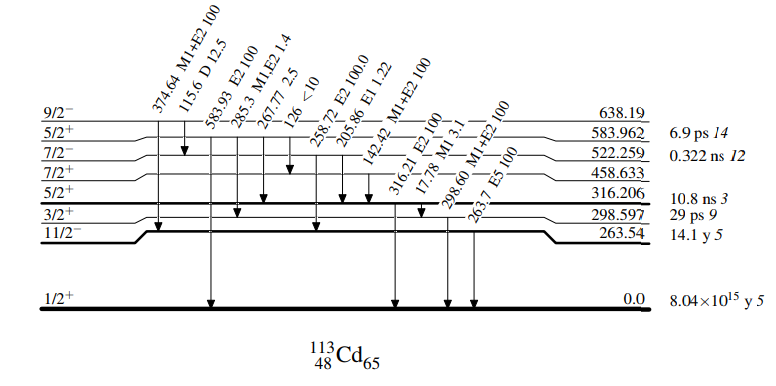
\includegraphics[width=0.9\textwidth]{113cd_partial_level_scheme_ENSDF.png}
	\caption{Partial level scheme for $\ce{^{113}Cd}$. The isomeric state has an energy of 263.54~keV~\cite{blachot_notitle_111}.}
\label{fig:cd113}
\end{figure}

\medskip
\noindent
Figure~\ref{fig:cd113} does suggest that there are already possible pathways by which $\cdm$ could be excited into a more energetic state and then decay into the ground state.
For example, the isomer could be excited into the $7/2^-$ state at 522.259~keV.
If it then decayed via an E1 transition to the 316.206~keV state before undergoing an E2 transition to the ground state, this would release the 263.54 keV stored in the isomer.
However, only 1.22 E1 transitions occurs for every 100 E2 transitions from the $7/2^-$ state, so this pathway would not be strongly favoured and thus potentially not a reliable option for achieving isomer depletion. % check
There are other options within the level scheme of $\ce{^{113}Cd}$ shown in Figure~\ref{fig:cd113}, but they are each similarly flawed.
% Check this little tangent to make sure it is correct. Get AJ to pay attention to this when he reviews this proposal.

\medskip
\noindent
Yet, isomer depletion has been experimentally achieved for six nuclides, using a range of distinct mechanisms, such as exposing a sample containing significant isomer population to bremsstrahlung radiation, using Coulomb excitation on said sample, or initiating nuclear excitation by electron capture
~\cite{shaffer_innovations_2018}.
Thus, should a practical depletion pathway be found within $\ce{^{113}Cd}$, there are methods that could be explored to demonstrate isomer depletion within this nuclide.

% Description of relevant models? Shell model, Nilsson/deformed shell model, ...?

\section*{Project Description}
%Project description: need to think about this
The analysis techniques and software that will be used are all methods and programs that are commonly used by and familiar to the other members of my research group.
They are also well documented, so there is a wealth of experience that can be tapped into when queries regarding the processing of data inevitably arise.
$\ce{^{148}Ce}$ and $\ce{^{150}Ce}$ have been studied using La $\beta^-$ decay experiments, so analysis of the recorded data for these isotopes will build on existing knowledge and potentially verify tentative conclusions reached in previous works.
Contrastingly, $\ce{^{152}Ce}$ has only been studied via the spontaneous fission of $\ce{^{252}Cf}$, so analysing this nuclide via the $\beta$ decay of $\ce{^{152}La}$ should provide new information on its structure.
Dedicated octupole collectivity studies have not been performed for any of these Ce isotopes, however, so this project will be breaking new ground in this area.
% Too grandiose?

\medskip
\noindent
By using $\beta$-$\gamma$ and $\beta$-$\gamma$-$\gamma$ coincidence analysis methods the program ROOT will be utilised to explore the recorded gamma ray data.
This process will enable the construction of a level scheme for each Ce isotope studied, aided by the consideration of $\gamma$-$\gamma$ coincidences (from the clover detectors) where one of the $\gamma$ rays is known to be emitted by a given Ce isotope.
Further analysis of gamma ray coincidences (as well as individual spectra) will then lead to the collection of key spectroscopic information, such as state lifetimes, excitation energies and spin-parities. %how for spin-parities?

\medskip
\noindent
If present, evidence of octupole collectivity will then be identified.
Primarily this be achieved by looking for strong E1 transitions between yrast bands of opposite parity, which will naturally require identification of the yrast bands themselves.
% How do we identify the yrast bands?
The strength of the octupole correlations that are present will then be assessed by evaluating the dipole and quadrupole moments of different transitions.
% Check that this is right, and how this actually works... I have no idea
For each Ce isotope, this will result in the fabrication of a level scheme that will contain some new levels, transitions and spectroscopic information, as well as an assessment of the degree of octupole collectivity that they each exhibit.

%This needs work/rewriting. See assessment sheet.
% Specifically, need to justify the methods chosen more clearly, and explain how this work fits into the field. This also holds for the octupole collectivity part - done for now.
% Need to highlight that the octupole collectivity stuff is new/original (based on the research proposal for the experiments themselves) whilst the cadmium stuff is largely just trying to build on what has been done before - done for now.
\medskip
\noindent
As for the nuclear isomer phase of this project, isomer depletion-focused studies of $\ce{^{113}Cd}$ have not yet been recorded.
Hence, at the very least, these tests will build upon existing knowledge of the level scheme of this nuclide (and potentially the phenomenon of break up as well).
Some prepatory work for this phase has already occurred.
The reactions that will be used have already been identified from a literature-based review of previous experiments that focused on excited states of $\ce{^{113}Cd}$.
The relevant reaction cross sections as a function of energy have also been calculated using the PACE4 fusion-evaporation code.

\medskip
\noindent
Should this phase go ahead, the detectors to be used in the CAESAR gamma ray detector array will need to have their energy resolution characterised, before they are inserted into the array.
Simultaneously, calculations will have to be performed to determine the parameters (beam energies, target thicknesses, exposure times) that are optimal for production and detection of excited states of $\ce{^{113}Cd}$.
Next, the targets will have to be readied, the experiments performed and then the data analysed. 
This data analysis will entail the construction of a level scheme, followed by the identification of any possible isomer depletion pathways.
Aside from the construction of the CAESAR array, I will be in charge of ensuring these steps are completed, with the help of other members of the ANU Nuclear Spectroscopy group as required.

\medskip
\noindent
Should time remain and charged particle detectors (fabricated and tested by other members of the Nuclear Spectroscopy group) be included in the CAESAR array, then it may also be possible to investigate breakup reactions that may have happened during the irradiation phase of the experiment.
This last step would extend the measured results of this project and would be interesting from a theoretical physics point of view, but is not required for the purpose of exploring isomer depletion.
However, if all of the other tasks above are completed, then a level scheme for $\ce{^{113}Cd}$ will be able to be constructed and potential depletion pathways identified. 


\section*{Project Plan and Feasibility}
% Insert Gantt chart with approximate deadlines.
% Could even be as approximate as going by month and just listing things to happen each month
% Data should be able to be accessed (via the server) from Friday 10 April.
% Current deadline for getting access to the lab again is 26 June.
\begin{figure}[htbp]
	\centering
	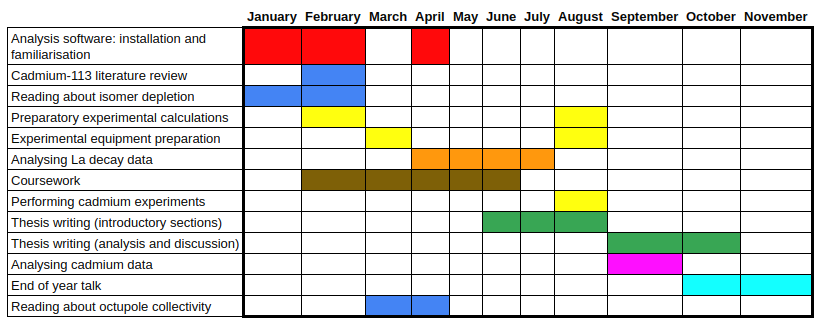
\includegraphics[width=0.9\textwidth]{GanttRP}
	\caption{Planned timeline for this project. The preparation for and performing of experiments in August represents the latest feasible time when this can occur. Tasks assigned to January through March have been completed.}
\label{fig:gantt}
\end{figure}
% room to tweak this for sure

\medskip
\noindent
The time allocated to each of the following steps is outlined in Figure~\ref{fig:gantt}.
The following data processing steps are central to the completion of a satisfactory project and will be performed using the ubiquitous nuclear data analysis frameworks ROOT and Radware.
\begin{enumerate}
\item Check the energy and time calibration of the existing gamma ray data.
\item Analyse the data in ROOT to construct a level scheme for $\ce{^{148,150,152}Ce}$.
\item Establish excitation energies and lifetimes of excited states in $\ce{^{148,150,152}Ce}$.
\item Identify the multipolarities and transitions between excited states of $\ce{^{148,150,152}Ce}$.
\item Measure the lifetimes of the $\ce{^{148,150,152}La}$ ground states and constrain their spin-parities (stretch goal).
\end{enumerate}
%Write introduction, motivation, background and methodology sections of thesis. I expect to finish these by August 31.

\medskip
\noindent
These analysis processes shall be continued in a dedicated manner until September 1 at the latest.
Concurrent to this analysis the writing of the introduction, motivation, background and methodology sections of the thesis shall occur. 
As time progresses, we will the feasibility of completing the planned $\ce{^{113}Cd}$ experiments before September 1 on a weekly basis.
This date is the latest feasible point at which there will remain time for thorough data analysis, collation of results and completion of the thesis, all by October 29.

\medskip
\noindent
If the restrictions on access to the accelerator building are lifted by August 1, then the steps below will be successively executed. The exact timing and feasibility will depend on beamtime being secured, through communication with my supervisor. All steps below are goals that are essential to the project unless otherwise specified.
%Dates somewhat arbitrary right now
\begin{enumerate}
\item Cool HPGe gamma ray detectors (for use in the CAESAR detector array) to liquid nitrogen temperatures.
\item Perform STROP calculations to identify the optimal target thickness, taking into consideration the energies identified as optimal for maximising the cross section for the reaction channel that produces $\ce{^{113}Cd}$.
\item Test HPGe detectors using PIXIE. Having already had some experience using this software, it will not take long to refresh my memory of how to use it.
\item Prepare $\ce{^{110}Pd}$ targets and create a mounting system for them. Establish whether we have enough targets and beamtime to perform experiments using both $\ce{^{7}Li}$ and $\ce{^{9}Be}$ beams.
\item Build the CAESAR detector array, in collaboration with various members of the Nuclear Spectroscopy group.
\item Perform experiments. Ideally we would perform experiments with both $\ce{^{7}Li}$ and $\ce{^{9}Be}$ beams, but this is time and target dependent. If limited beam time is available, only one beam may be used and the energy range utilised may be narrowed.
\item Analyse data to construct a level scheme for $\ce{^{113}Cd}$ and identify any viable depletion pathways.
Deduce all possible spectroscopic information.
The analysis skills gained during the octupole collectivity part of the project will enable this to be completed efficiently.
\item Stretch goal: analyse data to measure cross section for reactions performed as a function of energy.
\item Stretch goal \#2: If time permits, investigate charged particle-$\gamma$ coincidence data to explore any beam breakup reactions that occurred during the experiment(s).
\item Collate results and write results, discussion and conclusion sections of thesis. This will have to be completed by the deadline of October 29.
\item Prepare the final presentation, due November 5.
\end{enumerate}
This structure ensures that a satisfactory thesis will be generated from this project, but as it is the busiest possible timeline, provides plenty of room to omit parts should the time no longer be available for them.
While we hope to derive meaningful results from the data, if no such results are present, significant skills in the analysis of nuclear experimental data will have still been developed.
Thus the underlying goal of this project will be achieved no matter what happens.
% probably need to explain about how there are many reaction channels and not all of them are desired.

%Project plan: need to think about this
%
%Feasibility: Do-able. 

%\vspace*{-\baselineskip}
\bibliographystyle{ieeetr}
\bibliography{references.bib}{}
% No more than 20 refs


\end{document}